
\newcommand\epsilonzero{\si{\num{8.854E-12}\farad\per\meter}}
\newcommand\drivepotential{\si{\num{200}\volt}}


% STANDARD GEOMETRY

\section{A standard torsional oscillator}

\subsection{Geometry}
\label{sec.standard}
A common design used for torsional oscillators is shown in Figure~\ref{fig.StandardDesign}.
The oscillator is composed of a main body and a support rod. The main body contributes mostly to the total moment of inertia of the oscillator and usually contains the sample to study. The support rod acts as a spring and together with the moment of inertia, determines the natural resonance frequency of the oscillator.
\begin{figure}[htb]
	\captionsetup{width=.8\linewidth}
	\centering
	\includegraphics[width=7cm]{StdDesign1}
	\caption{ \small Common design of a torsional oscillator:
		The main body of the oscillator with the moving electrodes are shown in blue, the fixed electrodes in red, and the rod in green. A potential~$V_1$ is applied across capacitor~$C_1$ and a distinct potential~$V_2$ across~$C_2$.}
	\label{fig.StandardDesign}
\end{figure}
The oscillator is driven at resonance by a capacitor, and another one is used to measure its motion. Each of the capacitors is composed of two electrodes, one moving with the main body of the oscillator and the other one fixed in space. The main body of the oscillator is electrically connected to the moving electrodes and is grounded while any arbitrary potential can be applied to either of the fixed electrodes.

\subsection{Capacitance}
The geometry for of both capacitors is rectangular (see Figure~\ref{fig.StandardDesign2}).
\begin{figure}[htb]
	\captionsetup{width=.8\linewidth}
	\centering
	\includegraphics[width=9cm]{StdDesign2}
	\caption{ \small Cross section of the a capacitor: The }
	\label{fig.StandardDesign2}
\end{figure}
Both capacitor are almost identical except for the gap between the electrodes which can slightly differ due to construction. The capacitance value is given by the standard expression
\begin{equation}
C = \epsilon_0\frac{L H}{d}\,,
\end{equation}
where~$\epsilon_0$ is the vacuum permittivity ($\epsilon_0 = \epsilonzero $), $L$~and~$H$ are respectively the length and the height of the fixed plates, and~$d$ the distance (gap) between them. The value of $LH$ represents the overlapping surface area between the electrodes. This expression remains a good approximation as long as the distance between the capacitor plates stays small compared to the other dimensions: ($d\ll L$ and $d\ll H$).

\subsection{Energy}
When a static potential~$V$ is applied to one of the fixed capacitor plates, the electrostatic energy stored in the capacitor is:
\begin{equation}
U = \frac{1}{2}C V^2 =
\frac{1}{2} \frac{\epsilon_0 L H}{d} V^2 \,.
\end{equation}

\subsection{Force}
Therefore, the force exerted on the capacitor plates at a fixed voltage is\footnote{See: The Feynman Lectures on Physics, Volume II, Chapter 8 (Electrostatic Energy), paragraph 8.2 (The energy of a condenser. Forces on charged conductors).}:
\begin{equation}
F = \frac{1}{2} \frac{\epsilon_0 L H}{d^2} V^2 \,.
\label{Eq.ElecForce}
\end{equation}
This force always tends to reduce the distance between the capacitor plates.
In other words, the force is always attractive and does not depend on the sign of the potential~$V$.

\subsection{Displacement}
\label{sec.displacement}
% and $l$~is the distance from the centre of the electrodes to the axis of rotation.
When the fixed potential~$V$ is applied to the fixed electrode, the electric force~$F$ exerts a torque
\begin{equation}
\tau_1 = F l
\end{equation}
on the rod, where~$l$ is the distance from the centre of the capacitance plates to the axis of rotation. In reaction to the induced angular displacement~$\theta$, an opposite torque
\begin{equation}
\tau_2 = -\kappa \theta
\end{equation}
is produced by the elasticity of the rod. Here,~$\kappa$ is the torsional spring constant of the rod. For small angular displacements, we assume that the capacitor plates stay parallel and that we have approximately~$\theta \approx x/l$ where~$x$ is the change in the gap between the capacitor plates. At equilibrium we have $\tau_1+\tau_2 = 0$ such that:
\begin{equation}
\label{eq.static_equilibrium}
F l + \kappa \theta = 0\,.
\end{equation}
Replacing~$F$ by using~(\ref{Eq.ElecForce}) and~$\theta = x/l$, we get
\begin{equation}
\frac{1}{2} \frac{\epsilon_0 L H}{(d+x)^2} V^2 l + \kappa \frac{x}{l} = 0 \,.
\end{equation}
Since $x\ll d$, we can simplify to
\begin{equation}
x = - \frac{1}{2} \frac{\epsilon_0 L H V^2}{d^2} \frac{l^2}{\kappa} \,.
\end{equation}
Using a potential of~\drivepotential, an overlap area of~100mm$^2$
a gap on the order of \si{\num{100}\micro\meter} (giving a capacitance of 8.9pF), a typical torsion constant of \si{\num{3}\newton\meter} and a distance~$l$ of \si{\num{15}\milli\meter}, the displacement observed should be about~\si{\num{130}\nano\meter} which is 0.13\% of the gap (justifying our approximations).

\subsection{Driving force}
\label{sec.drive}
It appears from~(\ref{Eq.ElecForce}) that the force exerted on the capacitor plates is parabolic in~$V$. Hence, if we apply a harmonic potential~$V\propto \sin\omega t$ on the capacitor, the resulting force~$F\propto (1-\cos2\omega t)/2$ will have twice the frequency. In order to linearise~$F$, it is possible to add to the harmonic potential~$V$ a large static potential~$V_S \gg V$. In this case, the force applied on the electrode is
\begin{equation}
\frac{1}{2} \frac{\epsilon_0 L H}{d^2}
\left(V_S + V\right)^2 =
\frac{1}{2} \frac{\epsilon_0 L H}{d^2}
\left(V_S^2 + 2 V_S V + V^2\right) \\
= F_S + F + o(V^2) 
\end{equation}
% \frac{1}{2} \frac{\epsilon_0 L H}{d^2} V_S^2 +
% \frac{1}{2} \frac{\epsilon_0 L H}{d^2} V_S (2V + V^2)
where~$F_S$ is a constant (static) force
\begin{equation}
F_S = \frac{1}{2} \frac{\epsilon_0 L H}{d^2}V_S^2
\end{equation}
and $F$ is a harmonic driving force
\begin{equation}
F = \frac{\epsilon_0 L H}{d^2}V_S V
\label{Eq.OscDrive}
\end{equation}
linear in~$V$. The term~$o(V^2)$ is by design small compared to the other terms and has twice their frequency. It is neglected. The effect of the fixed term~$F_S$ is simply to shift the equilibrium position of the oscillator. The zero frequency response is obtained from~(\ref{eq.static_equilibrium}):
\begin{equation}
\label{eq.static}
x_0 = F \frac{l^2}{\kappa} = \frac{\epsilon_0 L H}{d^2} V_S V \frac{l^2}{\kappa} \,.
\end{equation}
Let's note that the factor~$V_S$ in~(\ref{Eq.OscDrive}) can be regarded as a useful amplification coefficient and that it can be easily boosted up in order to enhance the driving force amplitude.

Using a driving voltage of~\si{\num{5}\volt}, a static voltage of~\si{\num{200}\volt} and the other values as defined in Sec.~\ref{sec.displacement}, we obtain that~$x_0$ should be about~\si{\num{6.6}\nano\meter}.

\subsection{Resonance}
\label{sec.resonance}
The equation of motion of a driven oscillator can be expressed in the generic form
\begin{equation}
\ddot{\theta} + \lambda \dot{\theta} + \omega_0^2 (\theta -\theta_1 e^{i\omega t}) = 0 \,,
\label{Eq.HarmOsc}
\end{equation}
where the term~$\theta_1e^{i\omega t}$ is a sinusoidal drive which is here expressed in the same units as~$\theta$. The factor~$\lambda$ is a damping coefficient and~$\omega_0$ is the resonance frequency. This equation has harmonic solutions of the form
\begin{equation}
\theta=\theta_0 e^{i\omega t} \,,
\label{Eq.HarmonicSolution}
\end{equation}
where~$\theta_0$ is a complex number carrying the amplitude and the phase information. Replacing in~(\ref{Eq.HarmOsc}), we get the condition
\begin{equation}
\left(\omega_0^2 - \omega^2 + \lambda i \omega\right)\theta_0 - \omega_0^2\,\theta_1 = 0 \,.
\end{equation}
Defining the susceptibility~$\chi = \theta_0/\theta_1$, this can be rewritten
\begin{equation}
\chi = \frac{\omega_0^2}{\omega_0^2-\omega^2 + \lambda i \omega} =
\frac{\omega_0}{\lambda}\cdot \frac{1}{
\frac{\omega_0-\omega}{\lambda} \cdot
\frac{\omega_0+\omega}{\omega_0}+
i\frac{\omega}{\omega_0}} \,.
\label{Eq.Susceptibility}
\end{equation}
With the change of variable $\delta\omega = \omega - \omega_0$ which defines the departure from the resonance, it gives
\begin{equation}
	\begin{split}
	\chi & =  
		\frac{\omega_0}{\lambda}\cdot \frac{1}{
		\left(\frac{\omega_0-\omega_0 - \delta\omega}{\lambda}\right)
		\left(\frac{\omega_0+\omega_0 + \delta\omega}{\omega_0}\right)+
		i\left(\frac{\omega_0 + \delta\omega}{\omega_0}\right)}
	\\ & = 
		\frac{\omega_0}{\lambda}\cdot \frac{1}{
		-\frac{\delta\omega}{\lambda} \left(2 + \frac{\delta\omega}{\omega_0}\right) +
		i\left(1 + \frac{\delta\omega}{\omega_0}\right)} \,.
	\end{split}
\end{equation}
If the line width is small compared to the resonance frequency (which is the case in our oscillator: $\delta\omega/\omega_0\ll 1$), this reduces furthermore to
\begin{equation}
	\chi = \frac{\omega_0}{\lambda}\cdot \frac{1}{ -\frac{2\delta\omega}{\lambda} + i } \,.
\end{equation}
Pushing further by using the dimensionless variable~$\xi=2\delta\omega/\lambda$ and introducing the dimensionless quality factor~$Q=\omega_0/\lambda$, it takes the simplest form
\begin{equation}
	\chi/Q = \frac{1}{i-\xi} \,.
\end{equation}
This can be split into the real and an imaginary parts corresponding to the reactive and the dissipative terms of the resonance (See Figure.~\ref{fig.ResonanceCurve}):
\begin{equation}
	\chi_{\rm R}/Q = \frac{\xi}{1+\xi^2} \hspace{0.5cm} {\rm and}
	\hspace{0.5cm} \chi_{\rm D}/Q = \frac{1}{1+\xi^2} \,.
\end{equation}
\begin{figure}[h!]
	\captionsetup{width=.8\linewidth}
	\centering
	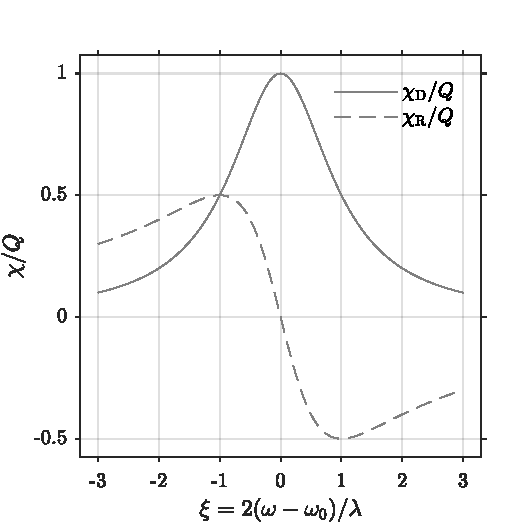
\includegraphics[width=0.7\linewidth]{resonancecurve}
	\caption{ \small Resonance curve in reduced units for $\omega_0/\lambda \gg 1$.}
	\label{fig.ResonanceCurve}
\end{figure}

The full width at half amplitude~$\Delta \xi$ is obtained for
\begin{equation}
	\frac{1}{1+\xi^2} = \frac{1}{2} 
	\hspace{0.5cm} \Leftrightarrow \hspace{0.5cm} \xi_{}\pm = \pm 1
	\hspace{0.5cm} \Leftrightarrow \hspace{0.5cm} \Delta \xi = 2\,.
\end{equation}
In non-reduced units this gives $\Delta\omega=\lambda$ and~$Q=\omega_0/\Delta\omega$. Experimentally the line width $\Delta\omega$ and the resonance frequency~$\omega_0$ are quantities easily measured.

Furthermore, from~(\ref{Eq.Susceptibility}) we can see that, at resonance when~$\omega=\omega_0$, we have~$\chi=\omega_0/\lambda$. From the same equation, when~$\omega\rightarrow 0$, we have~$\chi=1$. Thus the ratio between the zero frequency response and the response at resonance is~$\omega_0/\lambda=Q$. Hence, from~(\ref{eq.static}), we obtain the displacement amplitude at resonance:
\begin{equation}
\label{eq.amplitude}
x = Q\cdot x_0 = Q\cdot \frac{\epsilon_0 L H}{d^2} V_S V\frac{l^2}{\kappa} \,.
\end{equation}
Using the values from the previous sections and a typical quality factor~$Q$ on the order of~2500 at room temperature, we should obtain oscillations amplitudes on the order of~\si{\num{17}\micro\meter}.

\subsection{Velocity at resonance}
\label{sec.velocity}
The velocity of the oscillator follows directly from~(\ref{Eq.HarmonicSolution}):
\begin{equation}
\dot\theta=i\omega\theta_0 e^{i\omega t} = i\omega\theta
\end{equation}
Thus, in absolute values, at resonance, we obtain the velocity:
\begin{equation}
\label{eq.linearvelocity}
\dot x = l \dot \theta = l \omega_0 \theta = \omega_0 x 
=  \omega_0 Q \frac{\epsilon_0 L H}{d^2} V_S V\frac{l^2}{\kappa}
\end{equation}
From the values in the previous sections and a resonance frequency of~150Hz, we obtain a peak velocity on the order of \si{\num{16}\milli\meter\per\second}. If we can reach quality factors on the order of~50~000 at low temperatures, we should be able to reach the critical velocity of helium-II at about~\si{\num{300}\milli\meter\per\second}.

\subsection{Detection}
\label{sec.detection}
The detection relies on measuring the charge and discharge of our other capacitor when the potential is fixed and the gap~$d$ between the capacitor plates varies. For a fixed potential~$V_D$, the charge of the capacitor is given by
\begin{equation}
q  = C V_D = \frac{\epsilon_0 L H}{d+x} V_D
\end{equation}
where~$x$ is the deviation from the equilibrium position. The typical frequency of the oscillations is sufficiently low (typically 150Hz) so that the charging and discharging of the capacitor can be considered instantaneous. In this case, the charge depends only on the position of the capacitor plates and the current is given by
\begin{equation}
i = \dot{q}  = -\epsilon_0 L H\frac{\dot{x}}{(d+x)^2} V_D \,.
\end{equation}
Again, since the displacements are small compared to the gap ($x\ll d$) we can approximate to
\begin{equation}
i = -\epsilon_0 L H\frac{\dot{x}}{d^2} V_D \,.
\end{equation}
Using a current to voltage converter with a large gain~$G$, we obtain the velocity of the capacitor plates as a function of the measured amplifier output~$u$:
\begin{equation}
\label{eq.linearoutput}
\dot{x} = -\frac{d^2}{\epsilon_0 L H V_D} \frac{u}{G} \,.
\end{equation}
With a typical gain of~\si{\num{1d6}\volt\per\ampere}, $V_D=$~\si{\num{200}\volt} and using the values previously defined, a velocity of~\si{\num{1}\milli\meter\per\second} will give a typical signal on the order of \si{\num{18}\milli\volt}.

\section{Circular electrodes}
\label{sec.circular}
In the current design the maximum amplitude of oscillation is limited by the gap between the capacitor plates. At a peak velocity of~\si{\num{300}\milli\meter\per\second} the amplitude of the oscillations would reach~\si{\num{320}\micro\meter} which largely exceeds the gap value. Hence, a new design for the capacitors geometry has been devised in which the displacement between the capacitor plates is not transversal but parallel to the plates (see Figure~\ref{fig.CapacitanceDesignCircular}).
\begin{figure}[h!]
	\captionsetup{width=.8\linewidth}
	\centering
	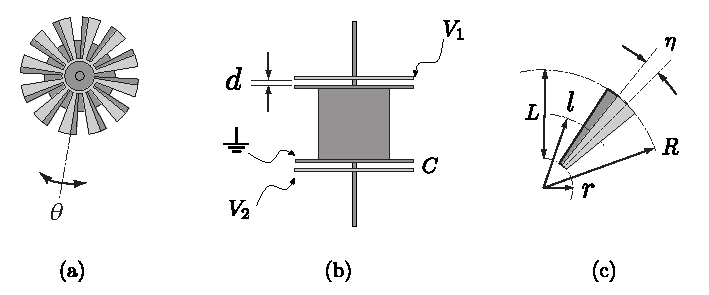
\includegraphics[width=12cm]{CircularCapacitanceValue2}
	% \includegraphics[width=12cm]{CapacitanceDesignCircular}
	\caption{ \small Capacitance geometry for a torsional oscillator with circular electrodes. (a) Top view of the oscillator. The moving parts are shown in dark grey. The fixed electrodes are shown in light grey. (b) Profile view of the oscillator showing the torsion rod and the gap between the capacitors plates. (c) Detail of the overlap geometry. The angle~$\eta$ is the overlapping angle between two facing electrodes.}
	\label{fig.CapacitanceDesignCircular}
\end{figure}
Each electrode is build from a set of smaller radial electrodes distributed in a star like fashion and connected by a small ring. The capacitance is formed using two plates facing each other and shifted by half an electrode width. Its capacitance is
\begin{equation}
C = \epsilon_0\frac{S}{d} =
\epsilon_0\frac{\pi(R^2 - r^2)}{d}\cdot\frac{\eta}{2\pi}=
\epsilon_0\frac{R^2 - r^2}{2d}\eta =
\epsilon_0\frac{L l}{d}\eta
\end{equation}
where~$L=R-r$ is the length of one electrode, $l=(R+r)/2$ the position of its centre from the axis of rotation and~$\eta$ the angle of overlap between the two electrode. For~$N$ electrodes in parallel, we find the total capacitor value:
\begin{equation}
\label{eq.circularCapacitance}
C = N \epsilon_0\frac{L l}{d}\eta \,.
\end{equation}
In contrast to the standard geometry, the gap between the circular electrodes is fixed and the change of capacitance is only due to variations of the overlapping angle during rotation. With 12 electrodes, $R = \si{\num{20}\milli\meter}$, $r = \si{\num{7.5}\milli\meter}$, giving $L = \si{\num{12.5}\milli\meter}$ and $l = \si{\num{13.75}\milli\meter}$, with a gap of~\si{\num{100}\micro\meter} and an overlap of \si{\num{6}\degree}, we expect a capacitance of~\si{\num{19.12}\pico\farad}.

\subsection{Energy and torque}
At a potential~$V$, the electric energy stored in the capacitor is
\begin{equation}
U = \frac{1}{2} C V^2 = \frac{1}{2} \epsilon_0 \frac{N L l}{d} \eta V^2 \,.
\end{equation}
Therefore, the torque applied on the oscillator is
\begin{equation}
\label{Eq.OscDrive2}
\tau_1 = \frac{1}{2}\epsilon_0 \frac{N L l}{d} V^2 \,.
\end{equation}
Note that the value of the torque is independent from the value of~$\eta$. This torque always tends to increase the overlap between the capacitor plates. In other words the plates tend to align with each other when an electric potential is applied.

\subsection{Static displacement}
In reaction to a displacement~$\theta$, the rod exerts in reaction a torque~$\tau_2 = -\kappa\theta$ leading to the equilibrium position
\begin{equation}
	\theta = \frac{1}{2}\epsilon_0 \frac{N L l}{\kappa d} V^2
\end{equation}
For a static potential of~\si{\num{200}\volt}, the displacement of the centre of the electrodes is $x = \theta l = \si{\num{16.7}\nano\meter}$.

\subsection{Harmonic drive}
Like the standard design, the force is still parabolic in~$V$. We can use the same method to linearise the force by adding a fixed voltage~$V_S$ much larger than~$V$ and we find the harmonic part of the driving torque
\begin{equation}
\label{Eq.drivetorque}
\tau = \epsilon_0\frac{NLl}{d}V_S V
\end{equation}
which is linear in~$V$. We then get the zero frequency response
\begin{equation}
	\theta_0 = \epsilon_0 \frac{N L l}{\kappa d} V_S V \,.
\end{equation}
Using \si{\num{5}\volt} for the drive we expect the displacement of the electrode centre to be $x_0 = \theta_0 l = \si{\num{0.84}\nano\meter}$. Compared with the standard design, this is about 8~times less.

\subsection{Harmonic displacement and velocity}
 From Section~\ref{sec.resonance}, we get the oscillator amplitude at resonance
\begin{equation}
\theta = Q \cdot \theta_0 = Q \cdot \frac{\epsilon_0 N L l}{\kappa d} V_S V
\end{equation}
and hence the oscillator velocity
\begin{equation}
\label{Eq.circularvelocity}
\dot\theta
= \omega_0 \cdot \theta
= \omega_0 \cdot Q \frac{\epsilon_0 N L l}{\kappa d} V_S V \,.
\end{equation}

This gives an amplitude of~$x = l \theta = \si{\num{2.09}\micro\meter}$ and a velocity of the centre of the electrodes ${\dot x} = l {\dot \theta} = \si{\num{1.97}\milli\meter\per\second}$.

\subsection{Detection}
From (\ref{eq.circularCapacitance}), we get the detection current
\begin{equation}
i = \dot C V_D = \frac{\epsilon_0 N L l}{d} V_D \dot\eta \,.
\end{equation}
Since ${\dot \theta} = {\dot \eta}$, we find the oscillator angular velocity from the voltage output~$u$
\begin{equation}
\dot \theta = \frac{d}{\epsilon_0 N L l V_D} \frac{u}{G} \,.
\label{eq.ThetaDotFromSignal}
\end{equation}
With a gain of~\si{\num{1d6}\volt\per\ampere}, we find that the output voltage is~\si{\num{2.67}\milli\volt} for a velocity of~\si{\num{1}\milli\meter\per\second}.

\subsection{Comparison}
A comparison between (\ref{Eq.OscDrive}) and (\ref{Eq.OscDrive2}) or between (\ref{eq.linearoutput}) and (\ref{eq.ThetaDotFromSignal}) leaves comparing the value of~$N$ and the value of~$H/d$. For $N=12$ and $H/d=100$, we expect the driving torque and the detection sensitivity to be roughly 8.3 times less in the case of the circular electrodes.

\section{Calibration and Estimation}
\subsection{Capacitance and gap}
The only value that is not directly measurable is the gap~$d$ between the electrode. It can be deduced on average from the measured capacitance if we have a good knowledge of~$\eta$. The error in the overlap can be estimated. We are using centring pins of diameter~$0.5$mm at a radius of~$20$mm at the moment of fixing the electrodes. This is equivalent to 1.43\si{\degree}. An overestimated error of half a pin diameter size gives an error of $\pm$12\% in the determination of the value of~$\eta$. From Section~\ref{sec.resonance}, we see that we can then estimate the average value of the gap to within~$\pm$14\% (inverse error).
\subsection{Measured velocity (from signal)}
In practice, we don't have to measure the gap to determine the velocity. From~(\ref{eq.ThetaDotFromSignal}), if we replace $d / \epsilon_0 N L l$ by~$\eta / C$ we see that the velocity of the oscillator at radius~$R$ is
\begin{equation}
v  = R \dot{\theta} = R\frac{\eta}{C V_D} \frac{u}{G}
\end{equation}
where all quantities are known or measured accurately except for~$\eta$. Therefore we can expect to know the velocity from the measured signal to within~$\pm$12\%.

\subsection{Expected velocity (from drive)}
The expected velocity is found from~(\ref{Eq.circularvelocity}). Replacing $\epsilon_0 N L l / d$ by~$C /\eta$, we get
\begin{equation}
v = R \left( \frac{\omega_0 Q}{\kappa} \right) \frac{C}{\eta} V_S V
\end{equation}
where the value of~$\kappa$ is not known with accuracy from the literature. However, the moment of inertia can be calculated with some certainty. From~$\omega^2_0 = k/I$ where~$I$ is the moment of inertia of the oscillator, we can rewrite
\begin{equation}
v = R \left( \frac{Q}{\omega_0 I} \right) \frac{C}{\eta} V_S V \,.
\end{equation}

\subsection{Oscillator constant}
The oscillator constant, so called "height, width over drive", can be calculated theoretically where the height is the signal output~$u$ in~[V], the width is the line width~$\Delta f = \Delta\omega/2\pi$ in~[Hz] and the drive is~$V$. This constant which is easily measured should be characteristic of the oscillator geometry and independent from the damping factors. From~(\ref{Eq.circularvelocity}) and~(\ref{eq.ThetaDotFromSignal}) we have respectively
\begin{equation}
u = G\frac{C_1}{\eta}V_D\dot{\theta}
\end{equation}
and
\begin{equation}
\dot{\theta} = G\frac{Q}{\omega_0 I}\frac{C_2}{\eta}V_S V \,.
\end{equation}
where~$C_1$ and $C_2$ are respectively the detection and drive capacitance. Replacing~$\theta$ and using~$Q=\omega_0/\Delta\omega$ gives
\begin{equation}
u\frac{\Delta f}{V} =
\frac{1}{2\pi I} \cdot \frac{C_1 C_2}{\eta^2} \cdot G V_D V_S
\end{equation}
with all quantities on the right hand side known or measurable independently. 
